% \documentclass[paper=a4, fontsize=11pt]{scrartcl} % A4 paper and 11pt font size
%
% \usepackage{hyperref}% in order to use hyperlinks
% \usepackage[T1]{fontenc} % Use 8-bit encoding that has 256 glyphs
% %\usepackage{fourier} % Use the Adobe Utopia font for the document - comment this line to return to the LaTeX default
% \usepackage[english]{babel} % English language/hyphenation
% \usepackage{amsmath,amsfonts,amsthm} % Math packages
% \usepackage{graphicx}
% \usepackage{epstopdf}
% \DeclareGraphicsExtensions{.eps}
% \usepackage{subcaption}
%
% %\usepackage{lipsum} % Used for inserting dummy 'Lorem ipsum' text into the template
%
% %\usepackage{sectsty} % Allows customizing section commands
% %\allsectionsfont{\centering \normalfont\scshape} % Make all sections centered, the default font and small caps
%
% \usepackage{fancyhdr} % Custom headers and footers
% \pagestyle{fancyplain} % Makes all pages in the document conform to the custom headers and footers
% \fancyhead{} % No page header - if you want one, create it in the same way as the footers below
% \fancyfoot[L]{} % Empty left footer
% \fancyfoot[C]{} % Empty center footer
% \fancyfoot[R]{\thepage} % Page numbering for right footer
% \renewcommand{\headrulewidth}{0pt} % Remove header underlines
% \renewcommand{\footrulewidth}{0pt} % Remove footer underlines
% \setlength{\headheight}{13.6pt} % Customize the height of the header
%
% \numberwithin{equation}{section} % Number equations within sections (i.e. 1.1, 1.2, 2.1, 2.2 instead of 1, 2, 3, 4)
% \numberwithin{figure}{section} % Number figures within sections (i.e. 1.1, 1.2, 2.1, 2.2 instead of 1, 2, 3, 4)
% \numberwithin{table}{section} % Number tables within sections (i.e. 1.1, 1.2, 2.1, 2.2 instead of 1, 2, 3, 4)
%
% \setlength\parindent{0pt} % Removes all indentation from paragraphs - comment this line for an assignment with lots of text
%
% %----------------------------------------------------------------------------------------
% %	TITLE SECTION
% %----------------------------------------------------------------------------------------
%
% \newcommand{\horrule}[1]{\rule{\linewidth}{#1}} % Create horizontal rule command with 1 argument of height
%
% \title{
% \normalfont \normalsize
% \textsc{CINVESTAV, Automatic Control Department} \\ [25pt] % Your university, school and/or department name(s)
% \horrule{0.5pt} \\[0.4cm] % Thin top horizontal rule
% \huge Benford's Law in Dynamical Systems \\ % The assignment title
% \horrule{2pt} \\[0.5cm] % Thick bottom horizontal rule
% }
%
% \author{Emanuel Rocha Campos, Gerardo E. Cardona S\'anchez} % Your name
%
% \date{\normalsize\today} % Today's date or a custom date
%
% \begin{document}

% \maketitle % Print the title

%----------------------------------------------------------------------------------------
%	PROBLEM 1
%----------------------------------------------------------------------------------------

\section{Overview}
The purpose of this document is to present the results of simulations and experiments regarding the implementation of a physical dynamical system, in this case, an autonomous electronic circuit made in order to look for Benford's Law conformity of a physical quantity. 
The circuits that were chosen for this objective have various regions of operation and can be easily regulated, so an important amount of experiments and simulations were performed.
Conformity to Benford's Law was achieved, and the circumstances under which the satisfactory results were obtained are also described in this document. 
%------------------------------------------------

\subsection{Benford's Law}
Benford's Law, also called the First Digit Law refers to the frequency distribution of digits from a data source.  The first observation was made by Benford \cite{Benford38} who looked through various sources of data and found that in some data sets the number 1 repeated about 30\% of the time, while larger digits occur less frequently. \\

Benford's Law is the probability distribution for the mantissa with respect to base $b \in \mathbb{N} \setminus \{1\}$ given by $\mathbb{P}(\text{mantissa}_b \leq t)=\log_b t  \forall t \in [1,b]$ ; the special case dealt with in this document is that described by:\\
\begin{align*}
    \mathbb{P}(\text{first significant digit}_{10} = d) = \log_{10}(1+\frac{1}{d})\text{,   }d=1,...,9
\end{align*}


Today, conformity to this distribution is looked for in accounting fraud detection\cite{Nigrini97}, election data and genome data. Moreover, a relationship between the brain electrical activity and Benford's Law was encountered, and the researches noted that compliance with Benford's Law is influenced by the presence of the anesthetic sevoflurane, or destroyed by noise in the EEG\cite{Kreuzer14}.

The following are two examples where Benford's Law holds: the well known Fibonacci sequence, and population data from Mexico's Municipalities, obtained from INEGI.


\subsubsection{Fibonacci Sequence}
The Fibonacci sequence consists in the sequence: 1,1,2,3,5,8,13,21,34,55,89,144, ... ; where the sequence can be defined as the recurrence relation:

\begin{align*} f_n=f_{n-1}+f_{n-2}\end{align*}

Next, the most significant digit from the first 1000 Fibonacci numbers is obtained, and the frequency of repetition of number 1 as the first digit is calculated, the same can be done with number 2, and so on until number 9. Finally a plot of this frequency distribution against the distribution predicted by Benford's Law is presented.


\begin{figure}[h]
\centering
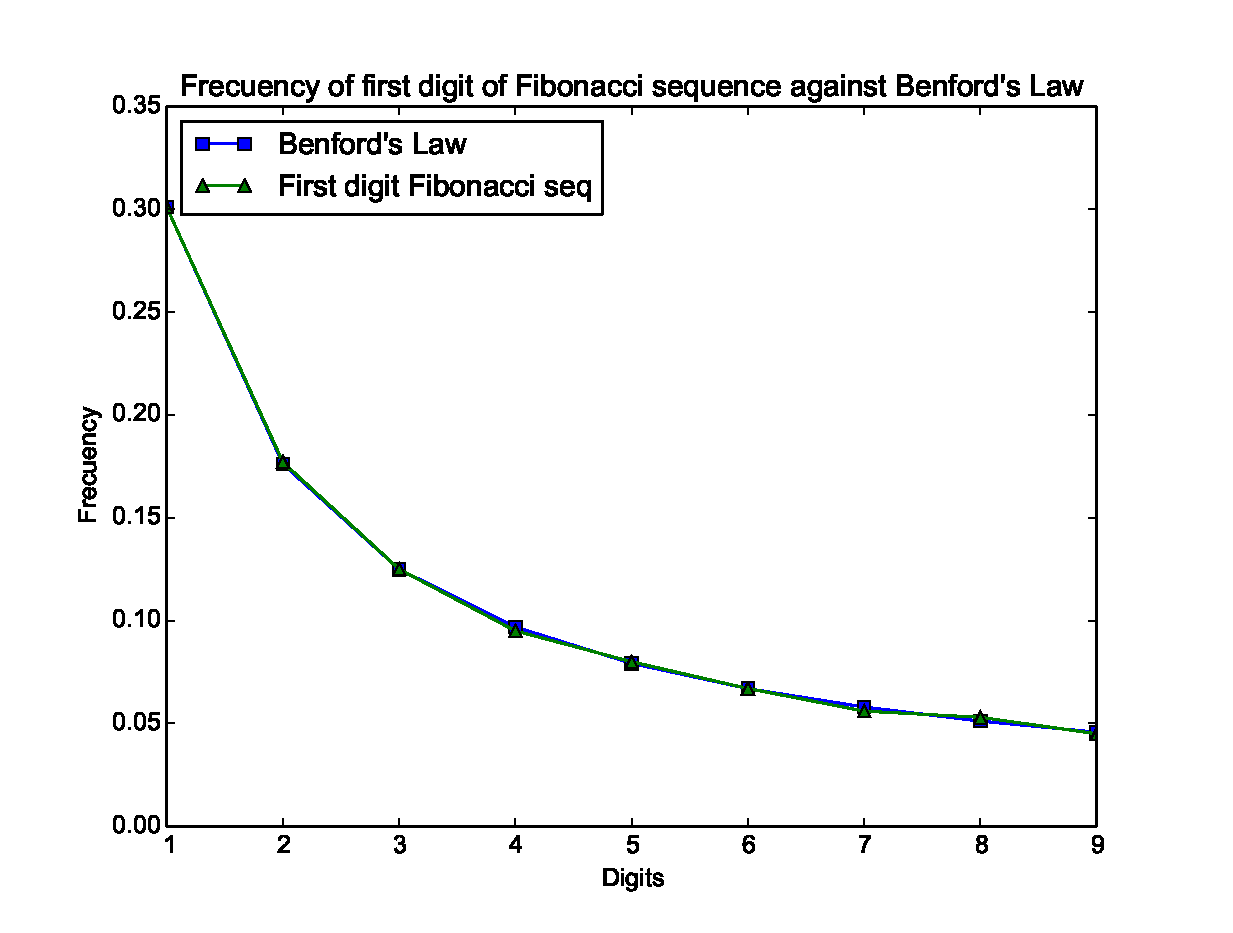
\includegraphics[scale=0.5]{imagenes/2-benford/benford_ex1}
\caption{Fibonacci Sequence against Benford's Law}
\end{figure}


\subsubsection{Mexico's Municipalities Population}
From the Mexico's National Institute of Geography and Statistics, INEGI, data from the 2010 census can be obtained. That year, 2351 Municipalities where censused and information is freely available at the institute web \href{http://www3.inegi.org.mx/sistemas/iter/entidad_indicador.aspx?ev=5}{page}.

As with the first example, the most significant digit of the population of each municipality was taken, and the frequency of repetition of each digit between 1 and 9 was compared with the prediction made by Benford's Law.

\begin{figure}[h!]
\centering
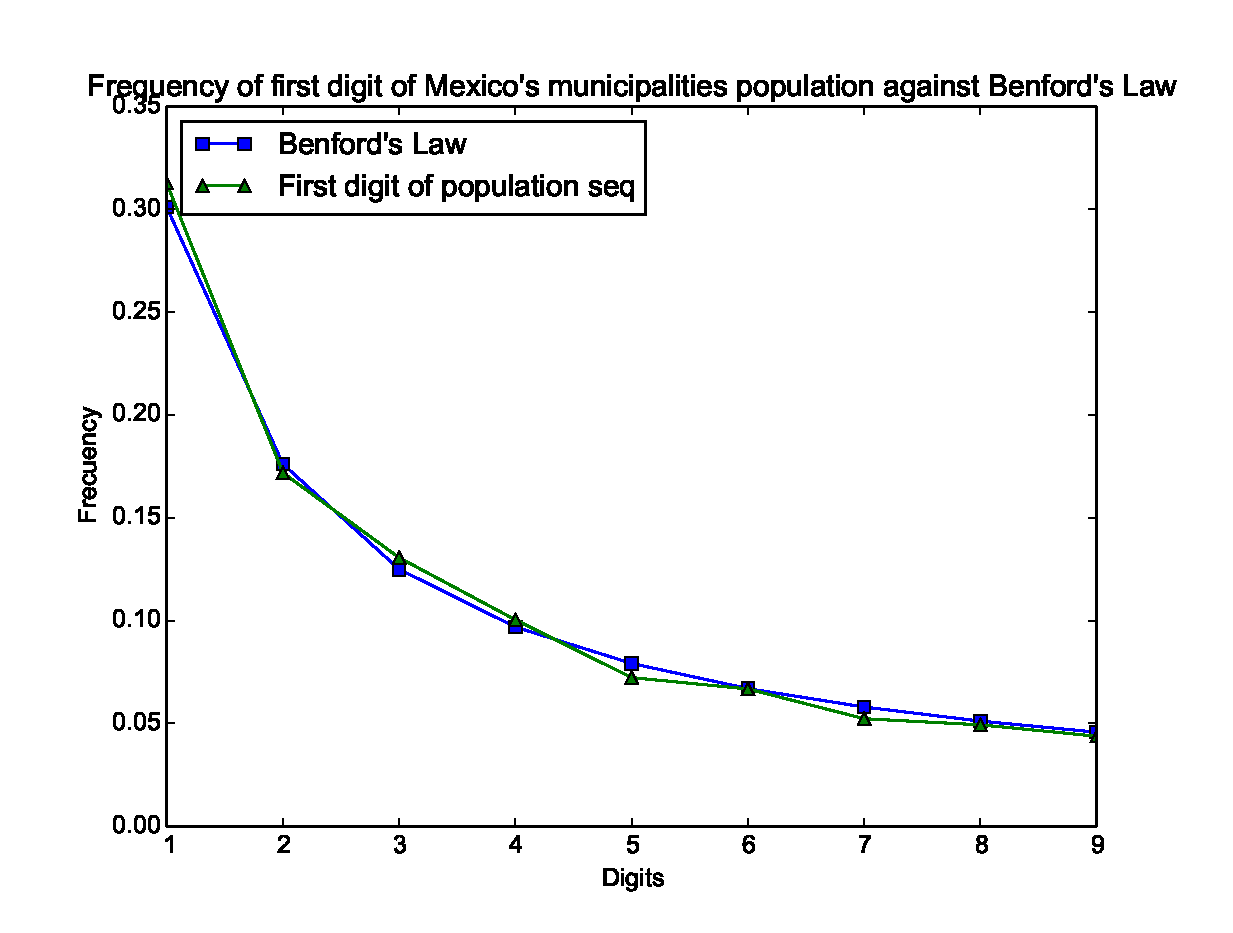
\includegraphics[scale=0.5]{imagenes/2-benford/benford_ex2}
\caption{Fibonacci Sequence against Benford's Law}
\end{figure}


\newpage
\subsection{Autonomous Circuits}
An Autonomous Circuit is a circuit that produces a time-varying output without having a time-varying input\cite{Kennedy95}. More formally:\\

An electronic circuit is described by a system of ordinary differential equations of the form:
\begin{equation*}
\dot{\mathbf{X}}(t)=\mathbf{F}(\mathbf{X}(t),t)
\end{equation*}
Where $\mathbf{X}(t)=(X_1(t),X_2(t),...,X_n(t))^T \in \mathbb{R}$ is called the \emph{state vector} and $\mathbf{F}$ is called the \emph{vector field}. $\dot{\mathbf{X}(t)}$ denotes the derivative of $\mathbf{X}(t)$ with respect to time.

If the vector field $\mathbf{F}$ depends explicitly on $t$, then the system is said to be \emph{non-autonomous}. If the vector field depends only on the state and is \emph{independent} of time $t$, then the system is said to be \emph{autonomous} and may be written in the simpler form:\\
\begin{equation}\dot{\mathbf{X}}=\mathbf{F}(\mathbf{X})\end{equation}


The time evolution of the state of an autonomous electronic circuit from an initial point $\dot{\mathbf{X}}$ at $t$=0 is given by\\

\begin{align*}\phi(\mathbf{X_0})=\mathbf{X_0}+\int_o^t\mathbf{F}(\mathbf{X}(\tau))d\tau &, t \in \mathbb{R}_+\end{align*}

The solution $\phi(\mathbf{X_0})$ is called a \emph{trajectory} through $\mathbf{X_0}$, and the set ${\phi(\mathbf{X_0}),t \in \mathbb{R}_+}$ is an \emph{orbit} of the system (1.1). The collection of maps ${\phi_t}$ that describe the evolution of the entire state space with time is called the \emph{flow}.

An autonomous electronic circuit is an example of a \emph{deterministic dynamical system}.

\subsection{Defining Chaos}
\emph{Chaos} is aperiodic long-term behavior in a determinisic system that exhibits sensitive dependence on initial conditions \cite{Strogatz14}
\begin{itemize}
\item \emph{Aperiodic long-term behavior} means that there are trajectories which do not settle down to fixed points, periodic orbits, or quasiperiodic orbits as $t$->$\inf$.
\item \emph{Deterministic} means that the system has no random or noisy inputs or parameters. The irregular behavior arises from the system's nonlinearity, rather than from noisi driving forces.
\item \emph{Sensitive dependence on initial conditions} means that nearby trajectories separate exponentially fast, i.e., that the system has a positive Lyapunov Exponent
\end{itemize}

\subsubsection{Lyapunov Exponent}
The lyapunov exponent of a dynamical system is a quantity that characterizes the rate of separation of infinitesimally close trayectories\cite{Parlitz92}.\\

Suppose that we let transients decay, so that a trajectory is \emph{on} the attractor. Suppose $\mathbf{\phi}(x,t)$ is a point on the attractor at time $t$, and consider a nearby point $\mathbf{\phi}(t)+\delta(t)$ where $\delta$ is a very small separation. It can be seen in the following figure, that  $\delta(t)$ grows. The two trajectories diverge with at a rate given by

$\lVert\delta(t) \rVert \ \lVert\delta_oo \rVert e^{\lambda t}$


\begin{figure}[h]
\centering
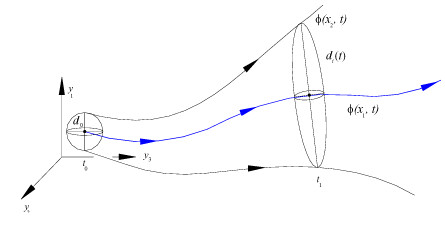
\includegraphics[scale=0.5]{imagenes/2-benford/Lyap_exp.jpg}
\caption{Neighboring trajetories separating exponentially fast with initial separation $\delta_0$ }
\end{figure}
When at least one Lyapunov exponent is positive the attractor possesses the property of sensitive dependence of initial conditions.


\subsubsection{Chua's Circuit}
\begin{itemize}\item \textbf{Chua's Oscillator}
\newline Leon Chua did research regarding Lorenz's equations\cite{Ayrom86}\cite{Kennedy95}, and deviced a chaotic electronic circuit with only one non-linear element, which is a 5-segment piecewise-linear resistor.


\begin{figure}[h]
\centering
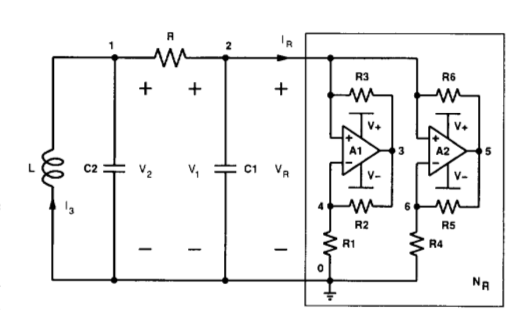
\includegraphics[scale=0.5]{imagenes/2-benford/chuas_circuit.png}
\caption{Schematic of Chua's Circuit }
\end{figure}

The dynamics of the system can be modeled by the system of three nonlinear ordinary differential equations:\\
\begin{align}
 \frac{dV_1}{dt}&=\frac{G}{C_1}(V_2-V_1)-\frac{1}{C_1}f(V_1)\\
 \frac{dV_2}{dt}&=\frac{1}{C_2}I_3-\frac{G}{C_2}(V_2-V_1)\\
 \frac{dI_3}{dt}&=-\frac{1}{L}V_2\\
\end{align}

with $G=\frac{1}{R}$ and $f(V_1)$ is given by:\\
\begin{align*}
\frac{G}{C1}V_2-\frac{G'_b}{C_1}V_1-(\frac{G_b-G_a}{C_1})E &\quad if \quad V_1< -E\\
\frac{G}{C1}V_2-\frac{G'_a}{C_1}V_1 &\quad if \quad -E\geq v1 \leq E\\
\frac{G}{C1}V_2-\frac{G'_b}{C_1}V_1-(\frac{G_a-G_b}{C_1})E &\quad if \quad V_1>E
\end{align*}
\item \textbf{Properties}
      \begin{enumerate}
       \item \textbf{Nonlinearity:} The system of equations has a nonlinear 2-terminal resistor described by a three segment piecewise-linear v-i characteristic shown in the following figure:


            \begin{figure}[h]
            \centering
            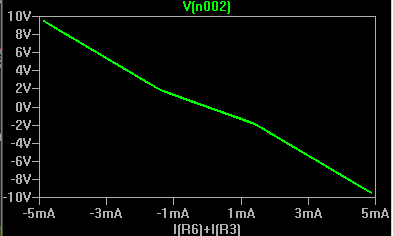
\includegraphics[scale=0.5]{imagenes/2-benford/v-i.png}
            \caption{v-i characteristic of the non-linear resistor }
            \end{figure}

      The piecewise-linear nature of the nonlinearity in Chua's Oscillator divides the state-space of the circuit into three distinct affine regions ($V_1<E$), ($\|V_1\|<E$) and ($V_1>E$)
      \item \textbf{Symmetry:}The piecewise-linear function is symmetric with respect to the origin, there exists three equilibrium points, at 0, $P_-$ and $P_+$. In the following figure, a double scroll Chua's attractor is shown. Since three equilibrium points are involved, this attractor is symmetric with respect to the origin\\

            \begin{figure}[h]
            \centering
            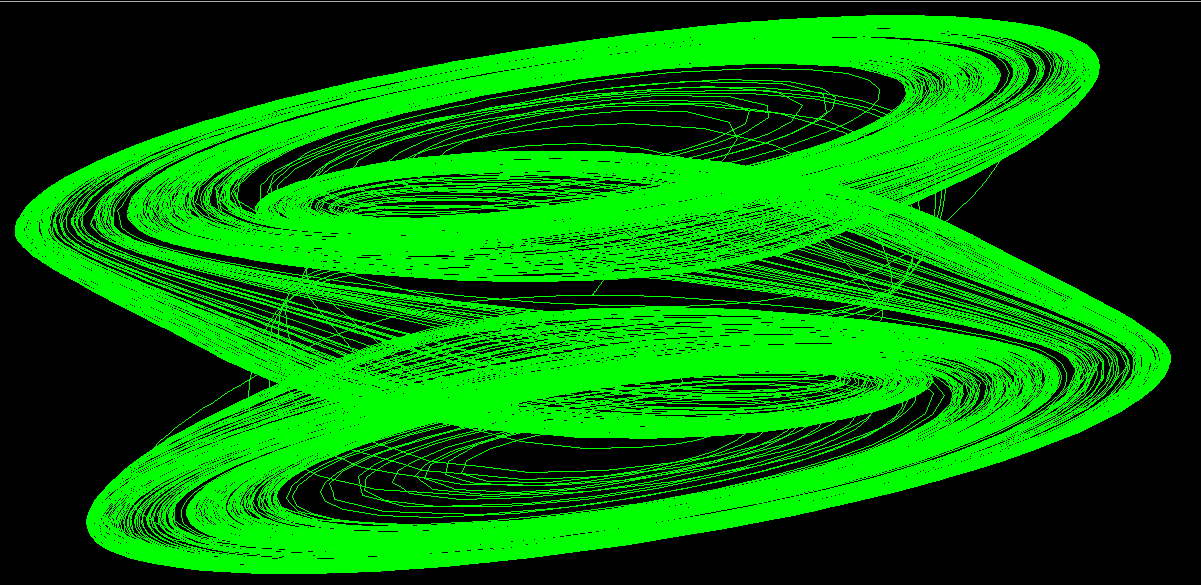
\includegraphics[scale=0.2]{imagenes/2-benford/chua_circuit.png}
            \caption{v-i characteristic of the non-linear resistor }
            \end{figure}
      \item \textbf{Dissipativity}
      \end{enumerate}
\end{itemize}


\newpage
\subsubsection{Takougang Circuit}
\begin{itemize}
\item \textbf{Three-dimensional autonomous system by Takougang et. al.}
    A three-dimensional autonomous system is presented by Sifei Takougang Kingni\cite{Takougang13}. The system exhibits chaotic bursting oscillations.\\
    The three-dimensional system is described as follows:\\
    \begin{align}
    \frac{dx}{dt}=-x+y\\
    \frac{dy}{dt}=xz-cy\\
    \frac{dz}{dt}=b-x^2-dz
    \end{align}

    where $b,c,d \in \mathbb{R}$
\item \textbf{Properties}
     \begin{itemize}
     \item \textbf{non-linearity:} Non-linearity given by the term $x^2$ and $xz$
     \item \textbf{symmetry:} Under the transformation defined by $(x,y,z) \rightarrow (-x,-y,-z)$, the system has a natural symmetry

     Next, we show that the system is symmetric.\\
     \textbf{Definition:}Let $f$ be a smooth function $f:\mathbb{R}^n \rightarrow \mathbb{R}^n$ and let\\
 \begin{align*}\mathbf{\dot{x}}=f(\mathbf{x})\end{align*}\\
 be a system of ordinary differential equations. In addition, let $\gamma$ be an invertible matrix. Then $\gamma$ is a \emph{symmetry} of the ordinary differential equation if \\
     \begin{align*}f(\gamma \mathbf{x})=\gamma f(\mathbf{x})\end{align*}

     Now, given the equation of the three-dimensional autonomous system, under the transformation $(x,y,z) \rightarrow (-x,-y,-z)$, to verify that this transformation is a symmetry of the autonomous equation, we observe that the symmetry is associated with the matrix $\gamma$ defined as\\
  \begin{align}
\gamma =
\begin{bmatrix}
-1 & 0 &0 \\
0 & -1 & 0\\
0 & 0 & 1
\end{bmatrix}
\end{align}

let \\  \begin{align}
\mathbf{\dot{x}}=f(\mathbf{x}) =
\begin{bmatrix}
-x + y \\
xz-cy\\
b-x^2-dz
\end{bmatrix}
\end{align}
with $\mathbf{x}^T=(x,y,z)$

Now, we proceed to show that $\gamma f(\mathbf{x})=f(\gamma \mathbf{x})$:\\
On the left hand side:
  \begin{align*}
\gamma f(\mathbf{x})&=
\begin{bmatrix}
-1 & 0 &0 \\
0 & -1 & 0\\
0 & 0 & 1
\end{bmatrix} \begin{bmatrix}
-x+y \\
xz-cy\\
b-x^2-dz
\end{bmatrix}\\
&=\begin{bmatrix}
x-y \\
-xz+cy\\
b-x^2-dz
\end{bmatrix}\\
\end{align*}

And now, on the right hand side:\\
  \begin{align*}
   f(\gamma \mathbf{x})&= f\left (\begin{bmatrix}
-1 & 0 &0 \\
0 & -1 & 0\\
0 & 0 & 1
\end{bmatrix} \begin{bmatrix}
x \\
y\\
z
\end{bmatrix} \right)\\
&=f\left ( \begin{bmatrix}
x \\
y\\
z
\end{bmatrix}\right )
&=\begin{bmatrix}
x-y \\
-xz+cy\\
b-x^2-dz
\end{bmatrix}
  \end{align*}

 Since the left hand side is equal to the right hand side, then $\gamma$ is a symmetry of the Three-dimensional Autonomous System. In other words, all solutions are either symmetric themselves, or have a symmetric partner
\item \textbf{Dissipativity} The system with the general condition for dissipativity (or Volume contraction):\\
         \begin{align*}\nabla V &= \frac{\partial(\frac{dx}{dt})}{\partial x}+\frac{\partial(\frac{dy}{dt})}{\partial y}+\frac{\partial(\frac{dz}{dt})}{\partial z}\\
&=-(1+c+d)
 \end{align*}

 So

\begin{align*}
V'(t)=-(1+c+d)V\\
V(t)V(0)e^{-(1+c+d)}t
\end{align*}

Thus volumes in phase space shrink exponentially fast
An explanation of dissipativity is given in \cite{Strogatz14} page 320.

\item \textbf{Fixed Points} The system has two types of fixed points:\\

      \begin{align*}
      0&=-x+y   \quad &\Rightarrow x=y\\
      0&=xz-cy   \quad&\Rightarrow z=c\\
      0&=b-x^2-dz  \quad&\Rightarrow x^2+dz=b \Rightarrow x=y=\sqrt{b-dc}
      \end{align*}
When $b \leq dc$ the fixed points for $x,y=0$ and $z=\frac{d}{b}$
When $b > dc$ the fixed points are $(\pm\sqrt{b-cd},\pm\sqrt{b-cd},c)$

\item \textbf{Sensitivity to initial conditons} Starting the system with slightly different initial conditions $(0, 0.1, 0)$ and $(0, 0.09, 0)$ we can see that after some time the two trajectories quickly diverge from each other



            \begin{figure}[h]
            \centering
            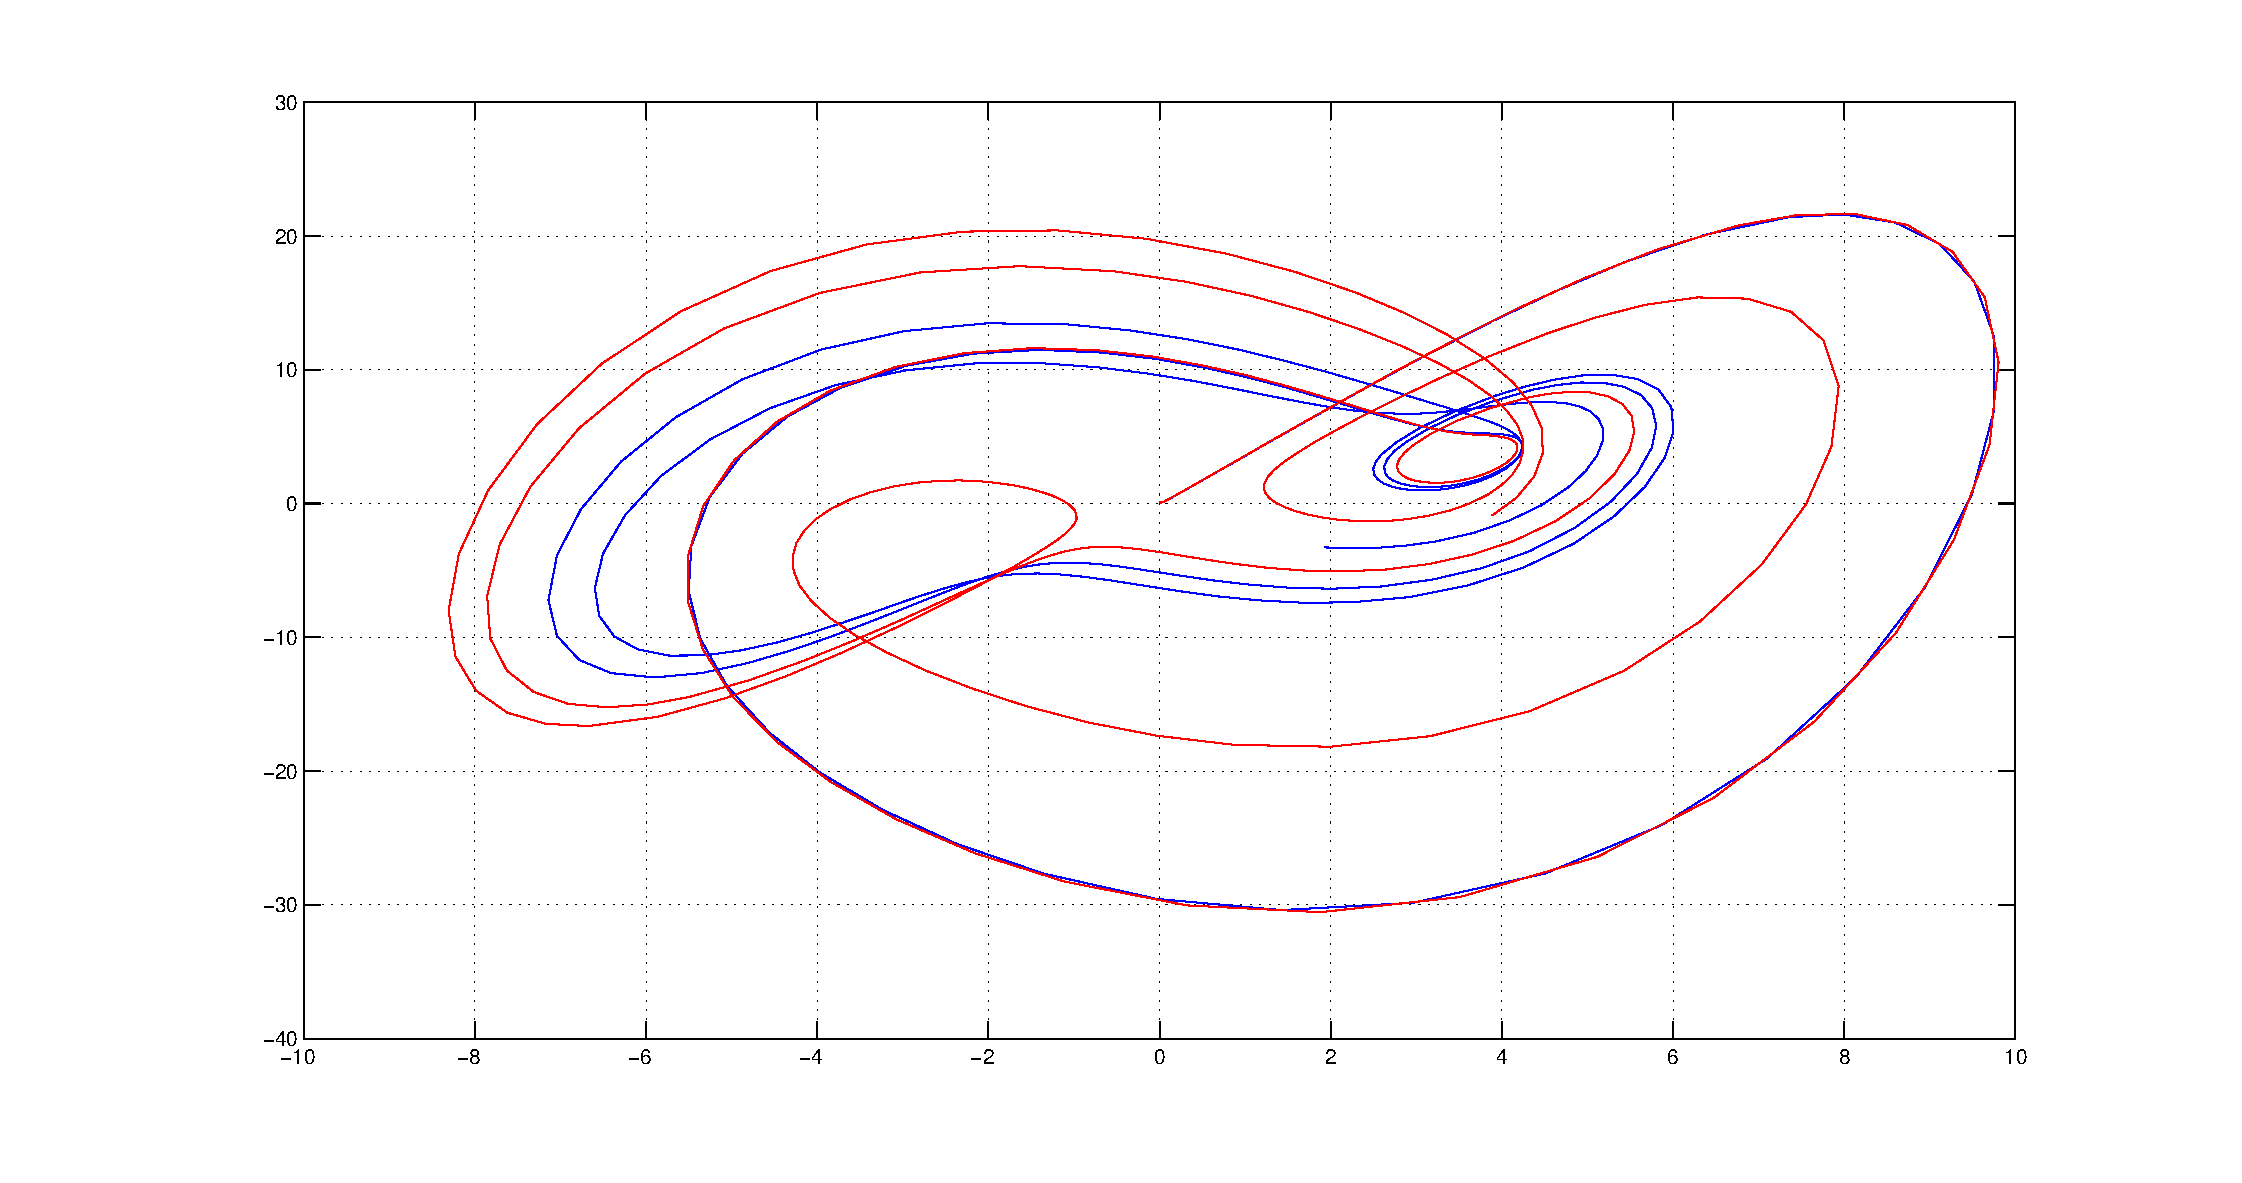
\includegraphics[scale=0.4]{imagenes/2-benford/in_cond.eps}
            \caption{Sensitivity to initial conditions in a Third Order Autonomous System}
            \end{figure}

     \end{itemize}
\end{itemize}

\cite{Takougang13} Shows that the system presents chaos of horseshoe type.


\newpage
\section{Simulations}
Simulations with Chua's System and the system proposed by \cite{Takougang13} were used to see if any of the system follows Benford's Law. On one hand we used Simulink and MATLAB in order to produce bifurcation diagrams and set up the dimensionless differential equations. On the other hand, we used a SPICE-based circuit simulator in order to get the systems in terms of electrical components.

\subsubsection{Chua's Circuit}
 \begin{itemize}
   \item \textbf{Physical Realization}
 The system describing chua's System
\begin{align*}
\frac{G}{C1}V_2-\frac{G'_b}{C_1}V_1-(\frac{G_b-G_a}{C_1})E &\quad if \quad V_1< -E\\
\frac{G}{C1}V_2-\frac{G'_a}{C_1}V_1 &\quad if \quad -E\geq v1 \leq E\\
\frac{G}{C1}V_2-\frac{G'_b}{C_1}V_1-(\frac{G_a-G_b}{C_1})E &\quad if \quad V_1>E
\end{align*}
is given by the following schematic
            \begin{figure}[H]
            \centering
            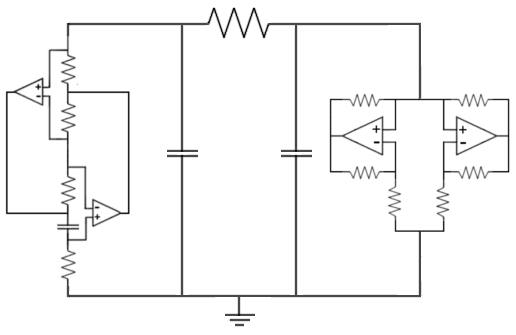
\includegraphics[scale=0.4]{imagenes/2-benford/chuas_circuit_realized.jpg}
            \caption{OP-Amp Based realization of Chua's Circuit}
            \end{figure}

With the Capacitors
C1=10nF
C2=100nF
and a 8mH Inductor given by the gyrator circuit.

   \item \textbf{Numerical Simulations}
   Using a spice based simulation software and MATLAB, several resistor values where tested, we constructed the bifurcation diagram and plotted for some R values
\begin{figure}
         \centering
            \begin{subfigure}[b]{0.4\textwidth}
            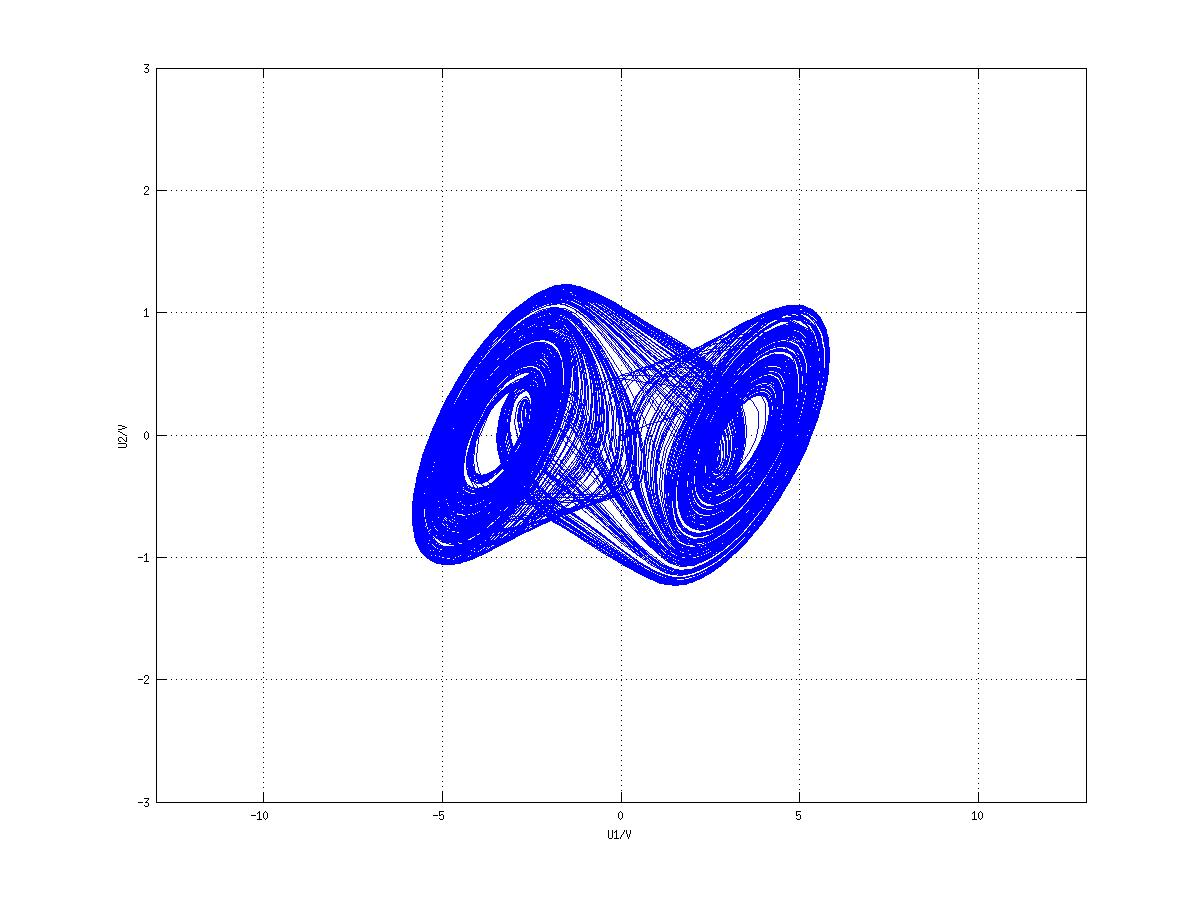
\includegraphics[width=\textwidth]{imagenes/2-benford/1785.jpg}
            \caption{V1-V2 plane for R=1785}
            \end{subfigure}
            \begin{subfigure}[b]{0.4\textwidth}
            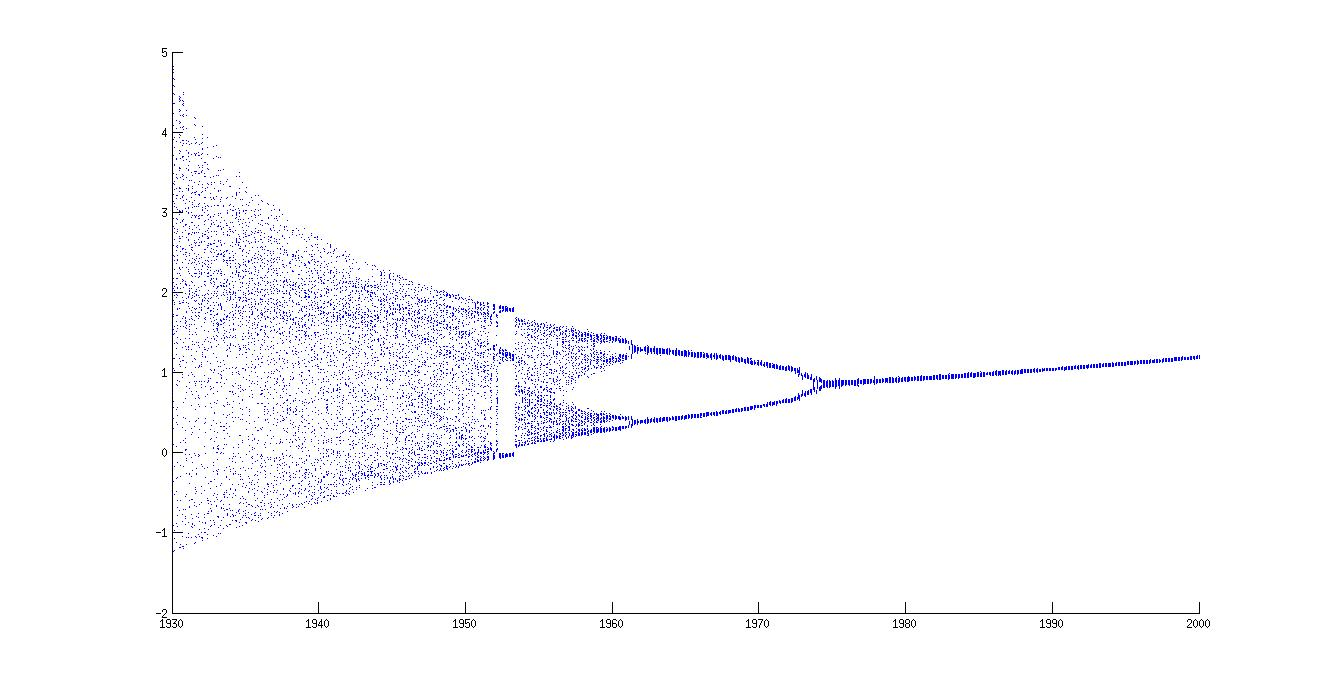
\includegraphics[width=\textwidth]{imagenes/2-benford/bifurcation_chua.jpg}
            \caption{Bifurcation Diagram for Chua's Circuit}
            \end{subfigure}
\end{figure}
   \item \textbf{Benford Analysis}
          The first digit distribution was determined from the voltage measured at the terminals of C1, using a resistance value of 1860$\Omega$, at that value, Chua's Circuit presented Chaotic Behaviour. The first digits (without leading zeroes) of the voltage values at discrete points were analyzed. We compared the first digit distribution of the dataset with the distribution given by Benford's Law using the Mean Absolute Deviation (MAD) proposed by \cite{Nigrini97}. We got a MAD value of 0.22, with a maximum of 0.15 in order to be conformant with Benford's Law.
            \begin{figure}[H]
            \centering
            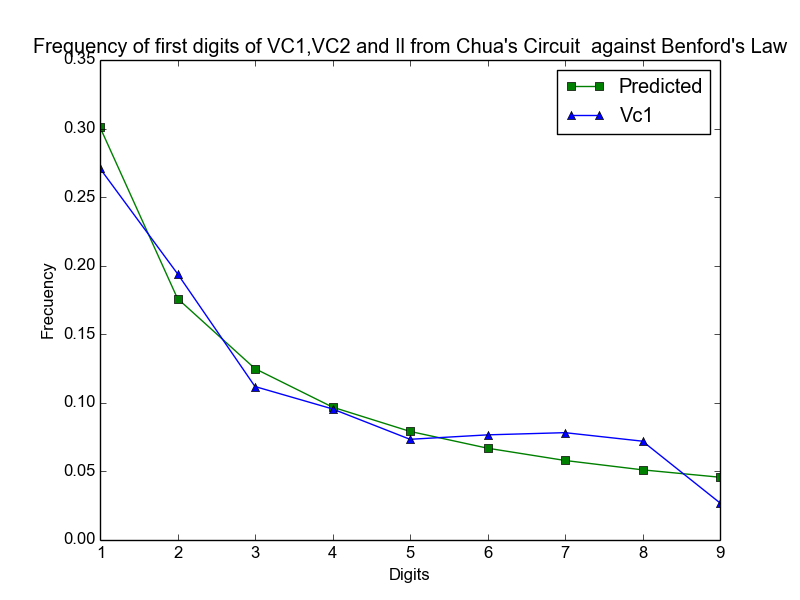
\includegraphics[scale=0.5]{imagenes/2-benford/chua_benford.png}
            \caption{OP-Amp Based realization of Chua's Circuit}
            \end{figure}
 \end{itemize}

\newpage
\subsubsection{Three-Dimensional Autonomous Circuit}
  \begin{itemize}
   \item \textbf{Physical Realization}
    The electronic circuit built to realise the system is shown in figure 2.4:
            \begin{figure}[H]
            \centering
            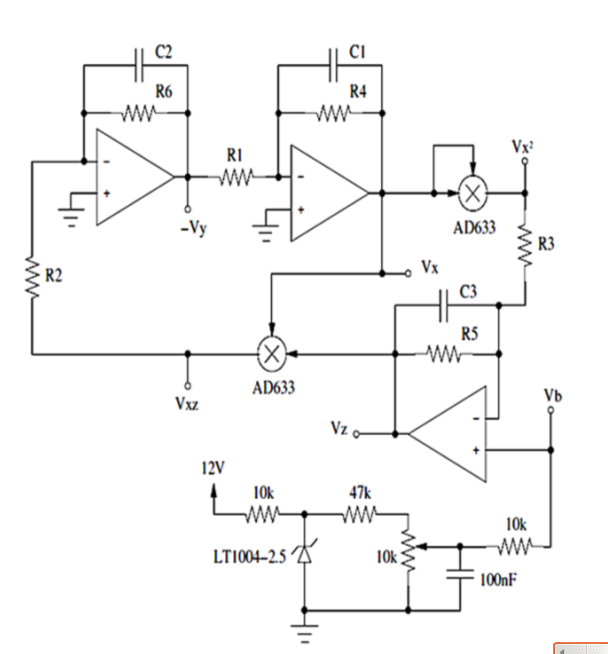
\includegraphics[scale=0.3]{imagenes/2-benford/Circuit2_schem.png}
            \caption{Circuit Schematic}
            \end{figure}
Voltages $V_x$,$V_y$ and $V_z$ are the output voltages of the operational amplifiers representing $x$,$y$ and $z$, $k_m=10V$ is the fixed constant of the AD633  multipliers, so the outputs of the multipiers are $V_{xz}=V_xV_z/k_m$ and $V_{x^2}=V_xV_x/k_m$.

            Substitution of resistor values into Eqs. (1.5),(1.6),(1.7) yields:

\begin{align}
\frac{dV_x}{dt}=\frac{1}{R_1C_1} \left ( V_y -V_x\frac{R_1}{R_4} \right )\\
\frac{dV_y}{dt}=\frac{1}{R_2C_2} \left ( \frac{V_xV_z}{k_m}-\frac{R_2}{R_6}V_y \right )\\
\frac{dV_z}{dt}=\frac{1}{R_3C_3} \left ( V_b\left ( 1+\frac{R_3}{R_5} \right )  -\frac{V_x^2}{k_m} - \frac{R_3}{R_5}V_z\right )
\end{align}

The values for resistors and capacitor used where: $R_1=0.5\text{ K}\Omega, \quad R_2=10\text{ K}\Omega, \quad R_3=10\text{ K}\Omega, \quad R_4=5\text{ K}\Omega, \quad R_5=1.15\textbf{\text{ M}}\Omega, \quad R_3=1\text{ M}\Omega, \quad C_1=100\text{ nF}, \quad C_2=100\text{ nF}, \quad C_3=10\text{ nF}, \quad V_b=10\text{ K}\Omega$
   \item \textbf{Numerical Simulations}
We used SIMULINK in order to model the system and MATLAB to create the bifurcation diagram.
            \begin{figure}[H]
            \centering
            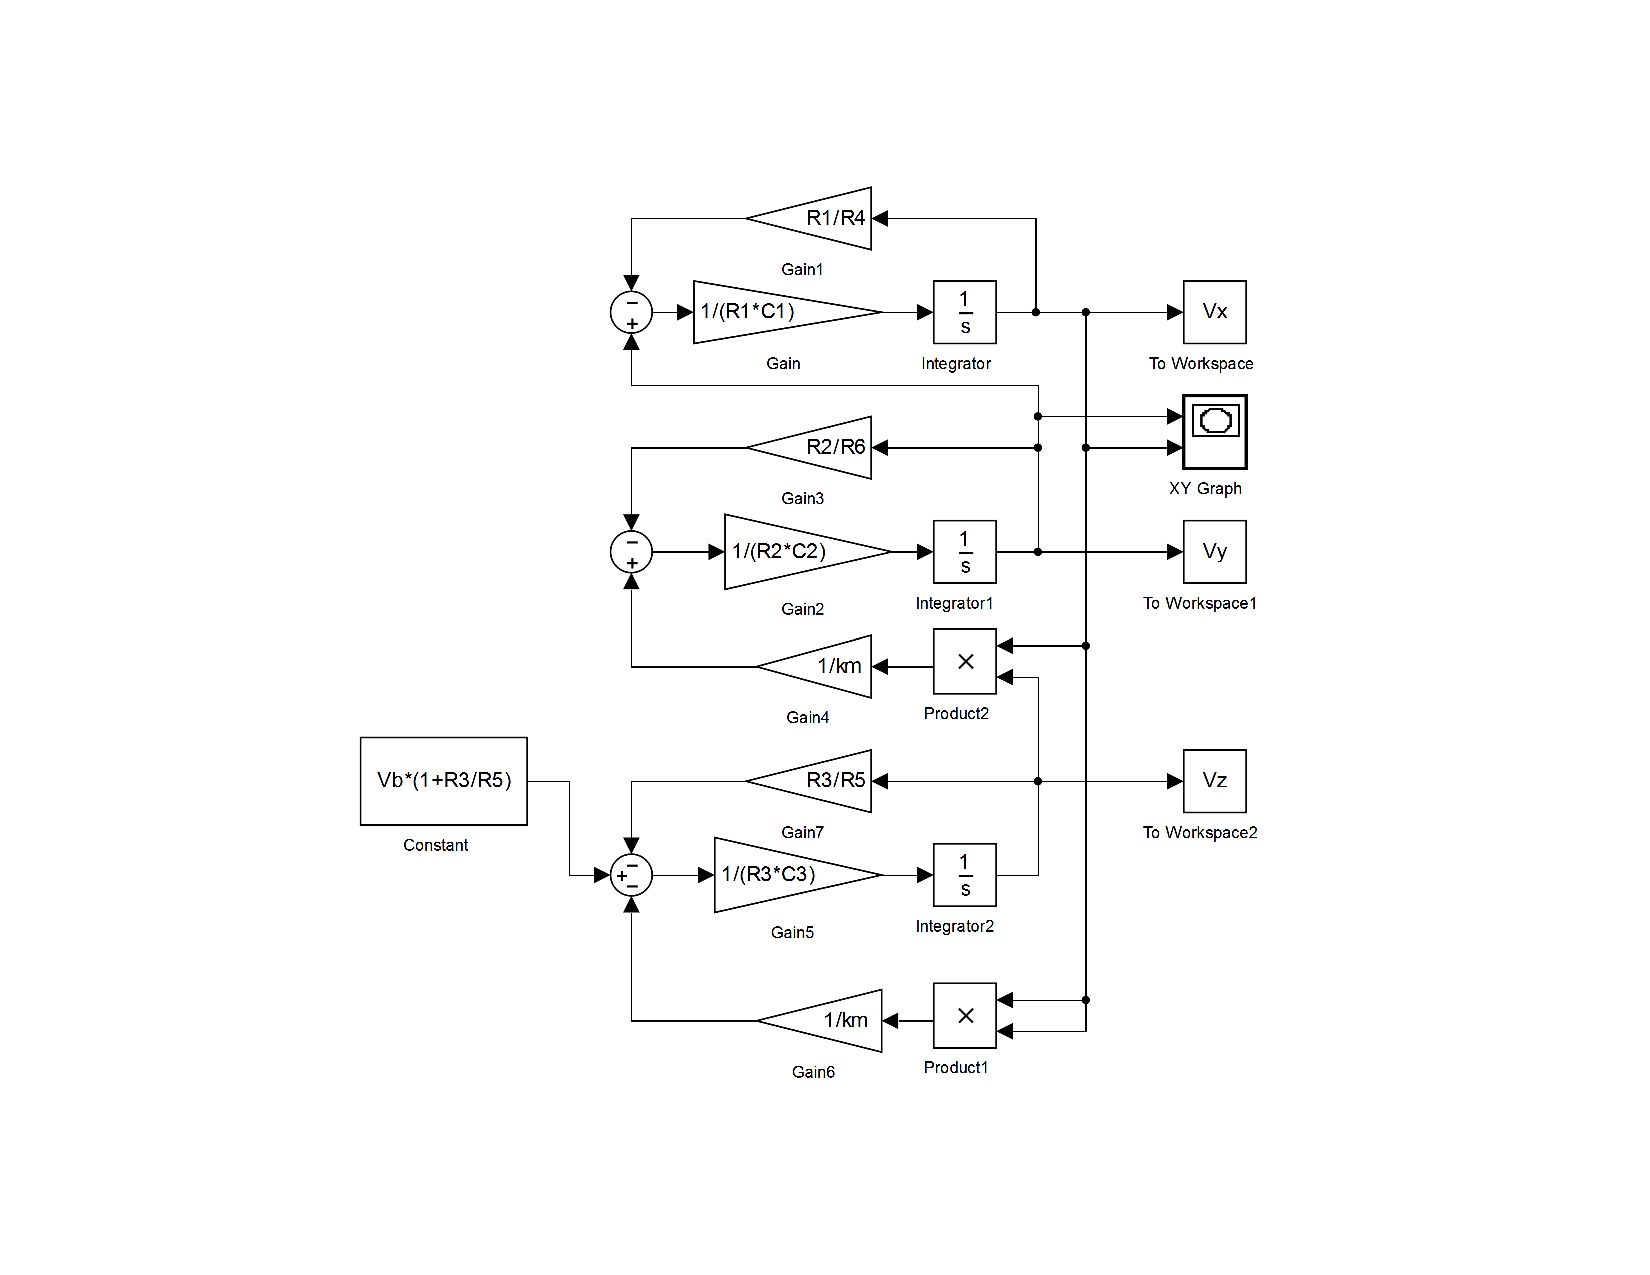
\includegraphics[scale=0.4]{imagenes/2-benford/shilkinovsimu.png}
            \caption{Simulink simulation}
            \end{figure}
The response of the syste with the parameters indicated above is given by figure 2.5:

\begin{figure}[H]
         \centering
            \begin{subfigure}[b]{0.4\textwidth}
            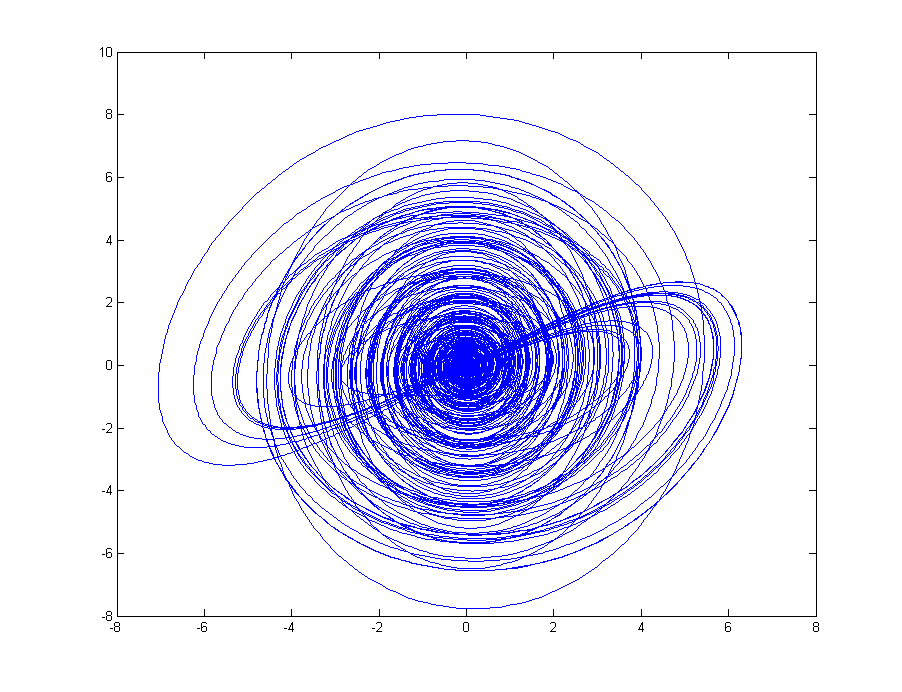
\includegraphics[width=\textwidth]{imagenes/2-benford/shilkino_resp.png}
            \caption{V1-V2 $V_x$ vs $V_y$ plot}
            \end{subfigure}
            \begin{subfigure}[b]{0.8\textwidth}
            \includegraphics[width=\textwidth]{imagenes/2-benford/bif_shil_osc_z.eps}
            \caption{Bifurcation Diagram varying b}
            \end{subfigure}
\end{figure}

Bifurcation diagram for the z value

   \item \textbf{Correspondence with Benford's Law} The same methodology used in Chua's Circuit was used with this circuit, taking measurements from $V_y$ and using the MAD test to verify conformity with the First Digit Distribution

            \begin{figure}[H]
            \centering
            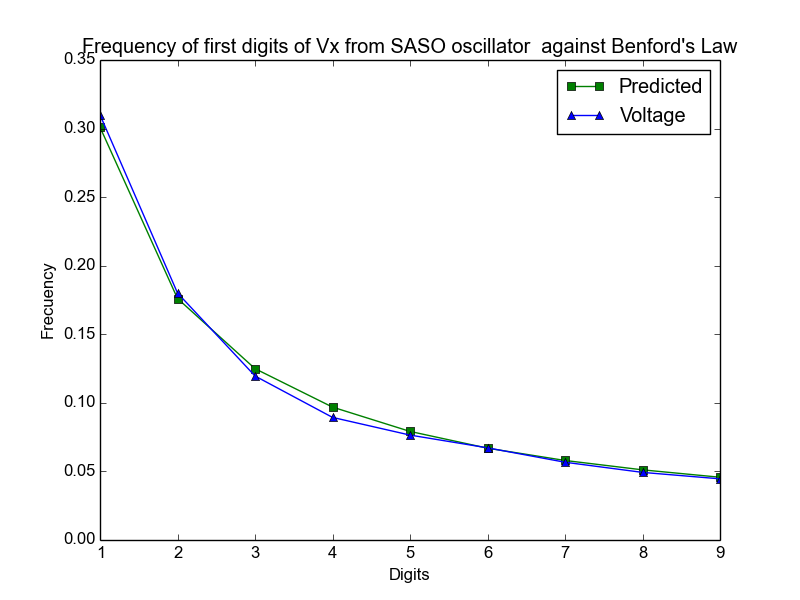
\includegraphics[scale=0.4]{imagenes/2-benford/Sh_vy.png}
            \caption{$V_x$ against Benford's Law}
            \end{figure}
For different values of d, we did a table with the respective first digit frequencies (10000 samples)  and MAD test.

\begin{center}
  \begin{tabular}{ c | c | c | c | c | c | c }
    \hline
    Leading digit  & Benford Distribution & d=1/23 &d=0.03 &d=0.01& d=0.001 &d=0.00001 \\ \hline
1&		0,3010&	0,3296&	0,3132&	0,3166&	0,2792&	0,3108\\ \hline
2&		0,1760&	0,1787&	0,1800&	0,1801&	0,1707&	0,1781\\ \hline
3&		0,1249&	0,1111&	0,1142&	0,1196&	0,1209&	0,1230\\ \hline
4&		0,0969&	0,0856&	0,0910&	0,0894&	0,0904&	0,0941\\ \hline
5&		0,0791&	0,0727&	0,0791&	0,0765&	0,0754&	0,0731\\ \hline
6&		0,0669&	0,0604&	0,0647&	0,0672&	0,0670&	0,0691\\ \hline
7&		0,0579&	0,0581&	0,0602&	0,0567&	0,0596&	0,0565\\ \hline
8&		0,0511&	0,0565&	0,0511&	0,0493&	0,0515&	0,0496\\ \hline
9&		0,0457&	0,0473&	0,0465&	0,0446&	0,0415&	0,0457\\ \hline
MAD&  & 0,0085&	0,0042&	0,0044&	0,0053&	0,0031\\ \hline

  \end{tabular}
\end{center}
We noticed strong agreement given by Nigrini\cite{Nigrini97}, next, we built the circuits and do tests measuring voltages.

 \end{itemize}


\newpage
\section{Experimental Results}
\subsubsection{Chua's Circuit}
 \begin{itemize}
  \item \textbf{Methodology}
We constructed the circuit using 4 TL082 I.C.'s and commercial resistors with the values used during simulation, Trimmer resistors to be able to move the resistor values of R.

            \begin{figure}[h]
            \centering
            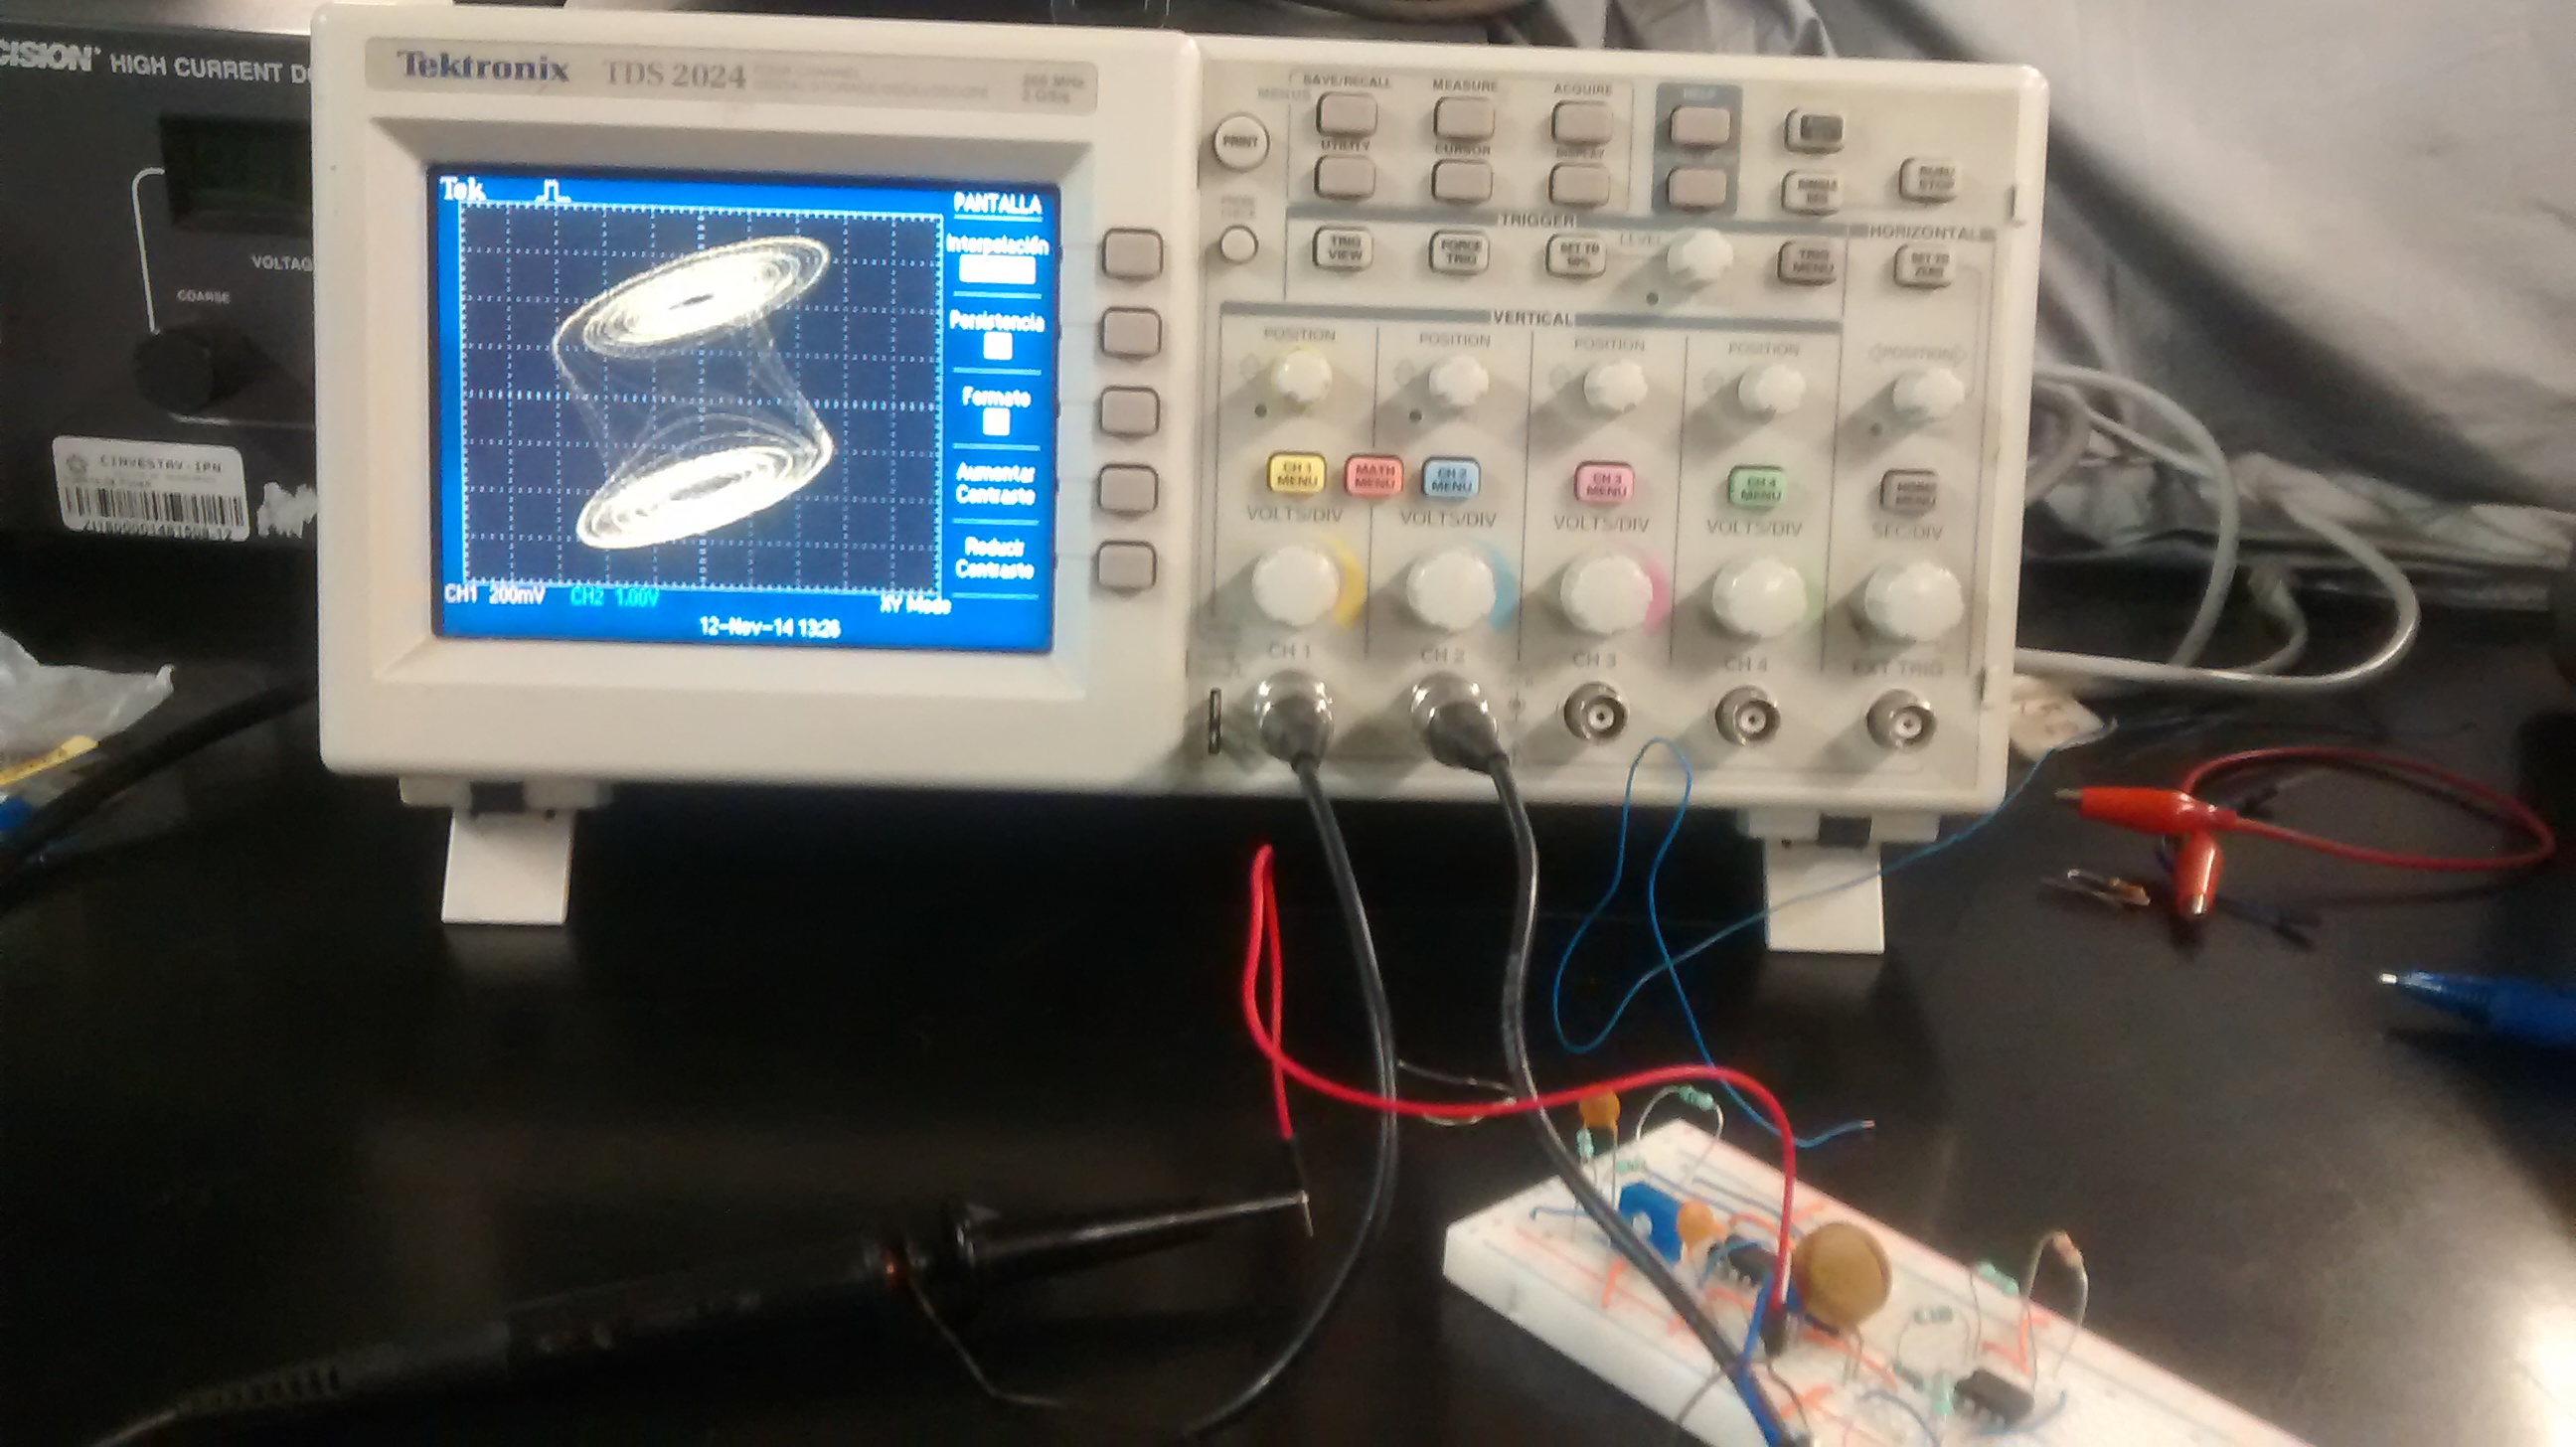
\includegraphics[scale=0.1]{imagenes/2-benford/chua_breadboard.jpg}
            \caption{Chua's System Breadboard}
            \end{figure}
We used two oscilloscope probes to measure the voltage from the two capacitors, and did our measurements with  a Tektronix DS201 Oscilloscope with a direct method sampling.

 The first digit distribution was determined from the voltage measured at the terminals of C1,varying R from 1700$\Omega$ to 1900$\Omega$in $25\Omega$ intervals, values in which Chua's Circuit presented chaotic behaviour. The first digits (without leading zeroes) of the voltage values at discrete points were analyzed, the oscilloscoped allowed us to take 2000 samples from a 250 $\mu$s period. We compared the first digit distribution of the dataset with the distribution given by Benford's Law using the Mean Absolute Deviation (MAD) proposed by \cite{Nigrini97}.



  \item \textbf{Results}
We put a table with the MAD results at each value of R:
\begin{center}
  \begin{tabular}{ c | c | c }
R & VC1 & VC2\\
1700 & 0.0265740826252 &0.0941252615083\\ \hline
1725 &  0.0308583854254& 0.0894910362566\\ \hline
1750 & 0.0225012003889 & 0.0937811348396\\ \hline
1775 &  0.0213932963068 & 0.0894482136018\\ \hline
1800 &  0.0515553953624& 0.0817178075546\\ \hline
1825 & 0.0620516456615 &0.0757908400412\\ \hline
1850& 0.0801858066881 &0.0616474503737\\ \hline
1875 & 0.0864648516751& 0.0566898036332\\ \hline
1900 &0.0848654579991 &0.0477795566486\\ \hline


  \end{tabular}
\end{center}

The closest value we got was with R=1775 measuring VC1
            \begin{figure}[h]
            \centering
            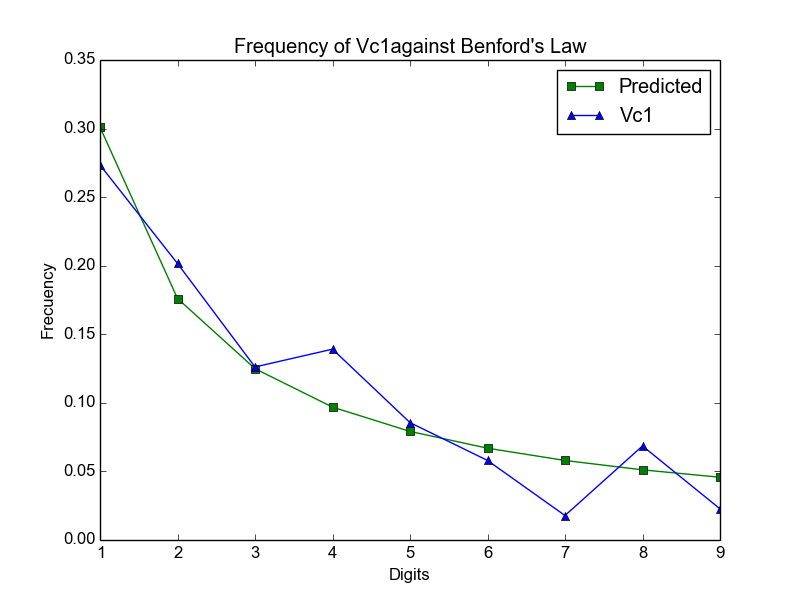
\includegraphics[scale=0.4]{imagenes/2-benford/benford_chua1775.png}
            \caption{Benford's Law against VC1}
            \end{figure}
  \item \textbf{Remarks}

We noticed that between for R between 1730 and 1775, there is a more clear First Digit Distribution according to Benford's Law, however, the measurements did not comply with MAD's Criteria which expects at most 0.015 in order to be compliant with Benford's Law. We also took a measurement with R=2000$\Omega$, value at which the system behaves as a quasi-periodic oscillator. we noticed that the first digit distribution is more uniform.

\begin{figure}
         \centering
            \begin{subfigure}[b]{0.4\textwidth}
            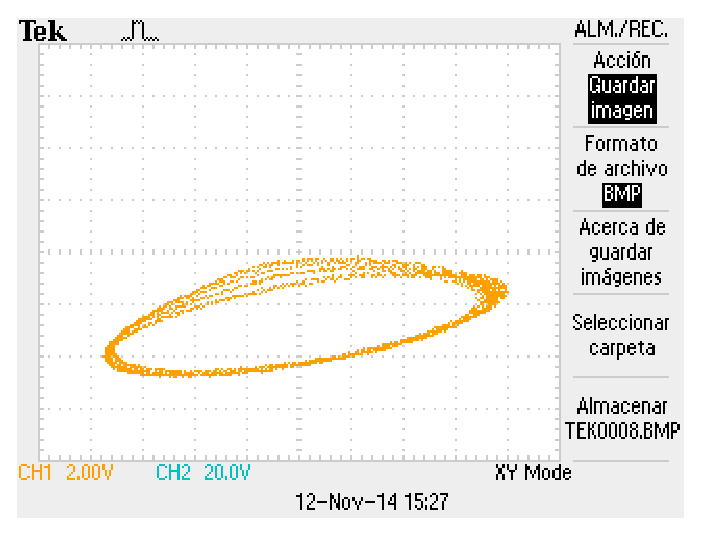
\includegraphics[width=\textwidth]{imagenes/2-benford/chua_2000.eps}
            \caption{V1-V2 $V_x$ vs $V_y$ plot}
            \end{subfigure}
            \begin{subfigure}[b]{0.8\textwidth}
            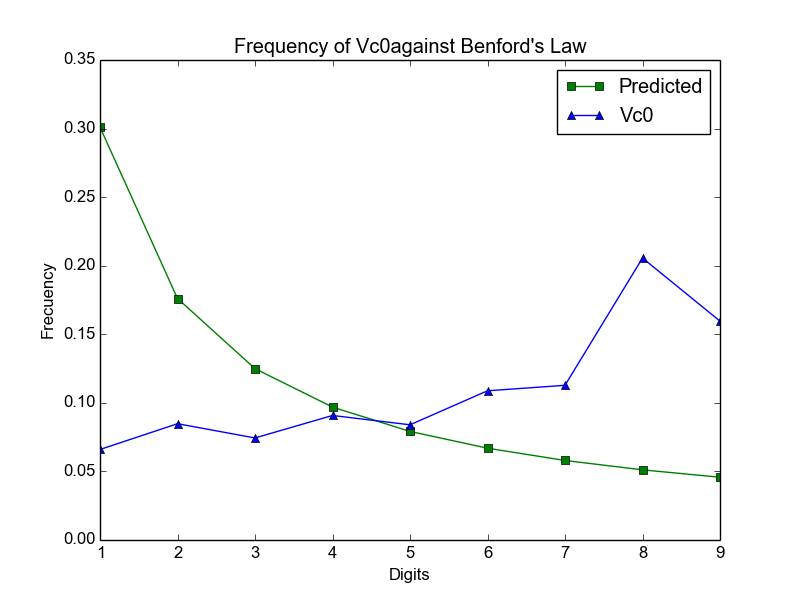
\includegraphics[width=\textwidth]{imagenes/2-benford/benford_chua20.png}
            \caption{Bifurcation Diagram varying b}
            \end{subfigure}
\end{figure}

 \end{itemize}
\subsubsection{Takougang Circuit}
 \begin{itemize}
  \item \textbf{Methodology}The circuit was connected using a standard breadboard, according to the diagram, all passive components had a nominal value equal to the ones proposed in the schematic, with a tolerance of 5\%. A regulated voltage source, set to $\pm$ 12 V was utilized to feed the active components which were the same as stated in the schematic. A third output of the regulated voltage source served to provide a stable input for the circuit ($V_b$). Next, a digital oscilloscope was used in order to obtain the data provided by the circuit.

A 1 GHz band-width oscilloscope (Agilent DSO6104A) was used next, and it was configured in order to reduce random noise. The sampler uses an averaging algorithm which delivers data with less noise, and reduces the vertical resolution (as low as 0.7 mV), with the data obtained from that oscilloscope the analysis was more reliable and results confirmed what was expected from the simulations, although only 1000 samples in an interval of 10 ms were fetched.
  \item \textbf{Results}
The first digit distribution of the voltages was taken and following the same methodology as with Chua's System, we swept through $V_b$ and took the MAD value from each distribution
\begin{center}
  \begin{tabular}{ c | c | c }
    \hline
$V_b$  & $V_x$&$V_y$\\ \hline
82mV & 0.0775279989288 & 0.0607280417648 \\ \hline
92mV & 0.0789296997697 &  0.0620760330126 \\ \hline
102mv & 0.0779822062934 & 0.0620098514762  \\ \hline
112mv & 0.0722551588234 & 0.0586329019652  \\ \hline
117mv & 0.0731369417692 & 0.0565637073089  \\ \hline
122mv & 0.0761361923841 & 0.0607646781498  \\ \hline
127mv & 0.0702382876578 & 0.0581541345311  \\ \hline
132mv & 0.0726371865346 & 0.0568562424256  \\ \hline
137mv & 0.0723923763659 & 0.0588608733569  \\ \hline
142mv & 0.0689722218274 & 0.0566979795649  \\ \hline
147mv & 0.0649140903028 & 0.0492049220995  \\ \hline
152mv & 0.0689575397758 & 0.0540809650999  \\ \hline
157mv &0.071269709088 & 0.0556102788266   \\ \hline
167mv &0.0713877270204 & 0.0546276659144  \\ \hline
187mv & 0.0642837364043 & 0.0499581746439  \\ \hline
197mv &0.0619961498144 & 0.0491763886427  \\ \hline
217mv & 0.0644054740322 & 0.0521147934116  \\ \hline
237mv & 0.0574813303354 & 0.0515391121266  \\ \hline
257mv & 0.0552768884655 & 0.0514296383228  \\ \hline
277mv & 0.0464325092508 & 0.0450451557158  \\ \hline
112mv (H-Res) &0.0126362748635 & 0.0149581584175  \\ \hline
132mv  (H-Res)& 0.0114562387312 & 0.0056682935093  \\ \hline
152mv  (H-Res)& 0.0106402668795 & 0.0143777130129  \\ \hline
172mv  (H-Res)& 0.0077090293797 & 0.0118696485616  \\ \hline
192mv  (H-Res)& 0.00801241025011 & 0.0120739312228  \\ \hline

  \end{tabular}
  \end{center}

We notice we have the best agreement with Benford's Law with $V_b=132mV$ Which gives a MAD value of 0.0056

            \begin{figure}[h]
            \centering
            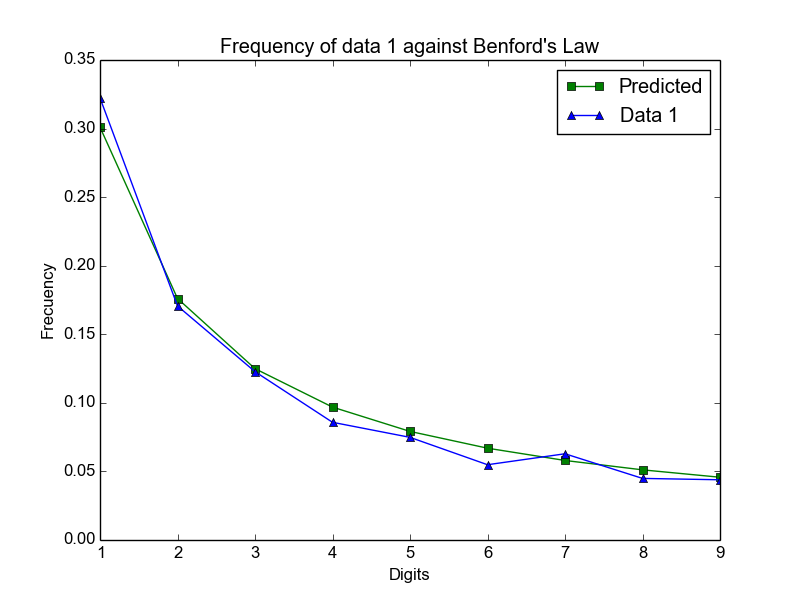
\includegraphics[scale=0.4]{imagenes/2-benford/benford_shilnikov_1.png}
            \caption{Benford's Law against digit distribution of $V_y$}
            \end{figure}

  \item \textbf{Remarks}

Simulations from Simulink gave a better accordance with $V_b=132mV$, however measuring without High-resolution sampling we did not obtain proper distributions, until we activated that sampling method, we got a distribution according to Benford's Law
 \end{itemize}


\section{Conclusion}
In the work done by Tolle \cite{Tolle00} some dynamical systems were proposed and theye checked if the first digit distribution followed Benford's Law. We took 2 autonomous circuits which displayed chaotic behaivour and verified if they were conformant according with the criterion given by Nigrini et. al. \cite{Nigrini97}. According to our experimental results, the system which best followed the distribution whas the Third Order Autonomous System proposed by Takougang et.al \cite{Takougang13}.

Verifyng the results from \cite{Takougang13}, we notice that this circuit has a Shilnikov heteroclinic orbit, which implies by the Shilnikov Criterion that the system has horseshoe chaos. This type of chaos produces time signals called chaotic bursting oscillations (see Fig. 4.1)
\begin{figure}[h]
            \centering
            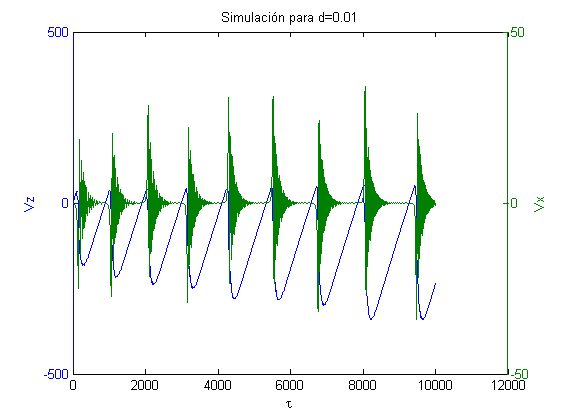
\includegraphics[scale=0.6]{imagenes/2-benford/bursting_oscilatons.png}
            \caption{$V_y$ response as a function of time}
            \end{figure}


This type of oscillations are found in biological phenomena, such as $Ca^2+$ oscillations in non-excitable cells \cite{Perc03}, pancreatic $\beta$ cells \cite{Sherman88} and in neurons\cite{Ermentrout09} and heart oscillatons, also, the work by Kreuzer et. al. \cite{Kreuzer14} indicates that brain electrical activity follows Benford's Law, so it would be interesting to see if Benford's Law could be an indicative if Real life phenomena is modelled correctly by the system if both follow Benford's Law (as it was first indicated by \cite{Tolle00}) and also to try to verify if other systems that present this kind of oscillations also follow Benford's Law.

%----------------------------------------------------------------------------------------
%  BIBLIOGRAPHY
\begin{thebibliography}{1}

\bibitem{Benford38}
  Benford Frank,
  \emph{The law of anomalous numbers}.
  Proc. Amer. Philos. Soc. 78,
  (1938),
  551-572.

\bibitem{Nigrini97}
  Nigrini Mark J., Mittermaier Linda J.
  \emph{The use of Benford's Law as an Aid in Analytical Procedures}
  Auditing: A Journal of Practice \& Theory,
  (1997),
  52-67

\bibitem{Kreuzer14}
  Matthias Kreuzer, Denis Jordan, PhD, Bernd Antkowiak, Berthold Drexler, Eberhard F. Kochs, and Gerhard Schneider
  \emph{Brain Electrical Activity Obeys Benford's Law}
  Neuroscience in Anesthesiology and Perioperative Medicine,
  (2014),
  183-191
\bibitem{Strogatz14}
 Steven H. Strogatz
  \emph{Nonlinear Dynamics and Chaos, With Applications to Physics, Biology, Chemistry and Engineering, Second Edition}
  Westview Press,
  (2014),
  309-191
\bibitem{Parlitz92}
  U. Parlitz
  \emph{Lyapunov's Exponent from Chua's Circuit}
  Journal of Circuits, Systems, and Computers,Vol. 3, No.2
  (1992),
  507-523
\bibitem{Kennedy95}
  Michale Peter Kennedy
  \emph{Experimental Chaos from Autonomous Electronic Circuits}
  Phil. Trans. R. Soc. Lond. A,
  (1995),
  507-523

\bibitem{Ayrom86}
Ayrom F.,
 \emph{Chaos in Chua's Circuit},
 IEE Proceedings, Vol. 133, No. 6 307-312
 , 1986,
 307-312


\bibitem{Takougang13}
Sifeu Takougang Kingni, Lars Keuninckx, Paul Woafo,  Guy Van der Sande, Jan Danckaert
\emph{Dissipative chaos, Shilnikov chaos and bursting oscillations
in a three-dimensional autonomous system: theory
and electronic implementation}
Nonlinear Dynamics,
2013

\bibitem{Torres07} Torres J. et al.,
 \emph{How do numbers begin? (The first digit law)},
  Eur. J. Phys., Vol. 28,
   2007,
   17-25

\bibitem{Tolle00}
Charles R. Tolle, Joanne L. Budzien, and Randall A. LaViolette
\emph{Do dynamical systems follow Benford’s law?}
Chaos: An Interdisciplinary Journal of Nonlinear Science 10,
 331,
2000
\bibitem{Perc03}
Perc, M., Marhl, M.
\emph{ Different types of bursting calcium
oscillations in non-excitable cells},
Chaos Solitons Fractals 18,
 759–773
2003
\bibitem{Sherman88}
Sherman, A., Rinzel, J., Keizer, J.
\emph{ Emergence of organized bursting in clusters of pancreatic $\beta$-cells by channel sharing},
Biophys. J. 54, 411–425,
1988
\bibitem{Ermentrout09}
\emph{Mathematical Foundations of Neuroscience}
Interdiscplinary Applied Mathematics 35,
103-126,
2009
\end{thebibliography}

% \end{document}
